\documentclass{article}
\usepackage{amsmath, mathtools}
\usepackage{amssymb}
\usepackage{tikz}
\usepackage{xspace}
\usepackage{float}
\usepackage{tabularx}
\usepackage{physics}
\usepackage{tikz}
\newcommand*\circled[1]{\tikz[baseline=(char.base)]{
   \node[shape=circle,draw,inner sep=1pt] (char) {#1};}}
\newcommand*\electron{\mathrm{e}^-}
\usepackage{paracol}
\usepackage[makeroom]{cancel}
\usepackage{makecell}

\title{AP Physics C: Chapter 25}
\author{Zach Baylin}

\begin{document}
  \maketitle
  \section{Intro to Electrodynamics}
    \begin{center}
      \begin{tabular}{c|c}
        Electrostatics & Electrodynamics \\ \hline
        Charge &  \checkmark\\
        insulator vs. conductor & \checkmark\\
        $F_E$ & \checkmark\\
        $\vec{E}$ & \checkmark\\
        $U_E$ & \checkmark\\
        $V$ & $\Delta V$ or $V$\\
        capacitors & batteries \\
         & $F_B$ \\
         & inductor 
      \end{tabular}
    \end{center}
    \begin{itemize}
      \item Circuit elements
        \begin{itemize}
          \item battery or capacity $\Delta V$
          \item wire (charge carrier)
          \item resistor
          \item inductor
          \item capacitor
        \end{itemize} 
      \item Equations
        \begin{itemize}
          \item \textbf{current ($I$)}: the rate of electron flow
            \begin{itemize}
              \item $I=\dfrac{\dd{Q}}{\dd{t}}$
              \item $I=N_E\cdot ev_d \cdot A$
              \item $I=\dfrac{\Delta V}{R}$ (for \textbf{ohmic materials})
            \end{itemize}
          \item \textbf{resistance ($R$)}: the tendency to resist current
            \begin{itemize}
              \item $R=\dfrac{\rho\ell}{A}$
              \item $R_{\mathrm{seq}}=\sum_i R_i$
              \item $R_{\mathrm{parallel}}^{-1}=\sum_i R_i$
              \item $\rho=I\Delta V$
            \end{itemize}
          \item \textbf{electric field ($\vec{E}$)}
            \begin{itemize}
              \item $\vec{E}=\rho\vec{J}=\rho\dfrac{I}{A}$
            \end{itemize} 
        \end{itemize}
      \item \textbf{electrodynamics}: controlled movement of charge in a conductor due to an \textit{internal} electic field
      \item the charge \textit{carrier} is what moves
        \begin{itemize}
          \item \underline{metal}
            \begin{itemize}
              \item $\electron$ bound to the solid, not individual atoms
              \item random thermal motion of $\electron$
              \item collisions with lattice
              \item net motion $=0$
              \item the electric field is like a push that causes all $\electron$ to have a direction
              \item \textbf{drift velocity ($v_d$)}: $v_d=\dfrac{\Delta x}{\Delta t}=10^{-4}m/s$
              \item \textbf{electron current ($i_e$)}: $i_e=\dfrac{n_e}{\Delta t}$
              \item \textbf{number of electrons ($N_e$)}: $N_e=\dfrac{n_e}{\mathrm{volume}}$
            \end{itemize}
            \begin{figure}[H]
              \centering
              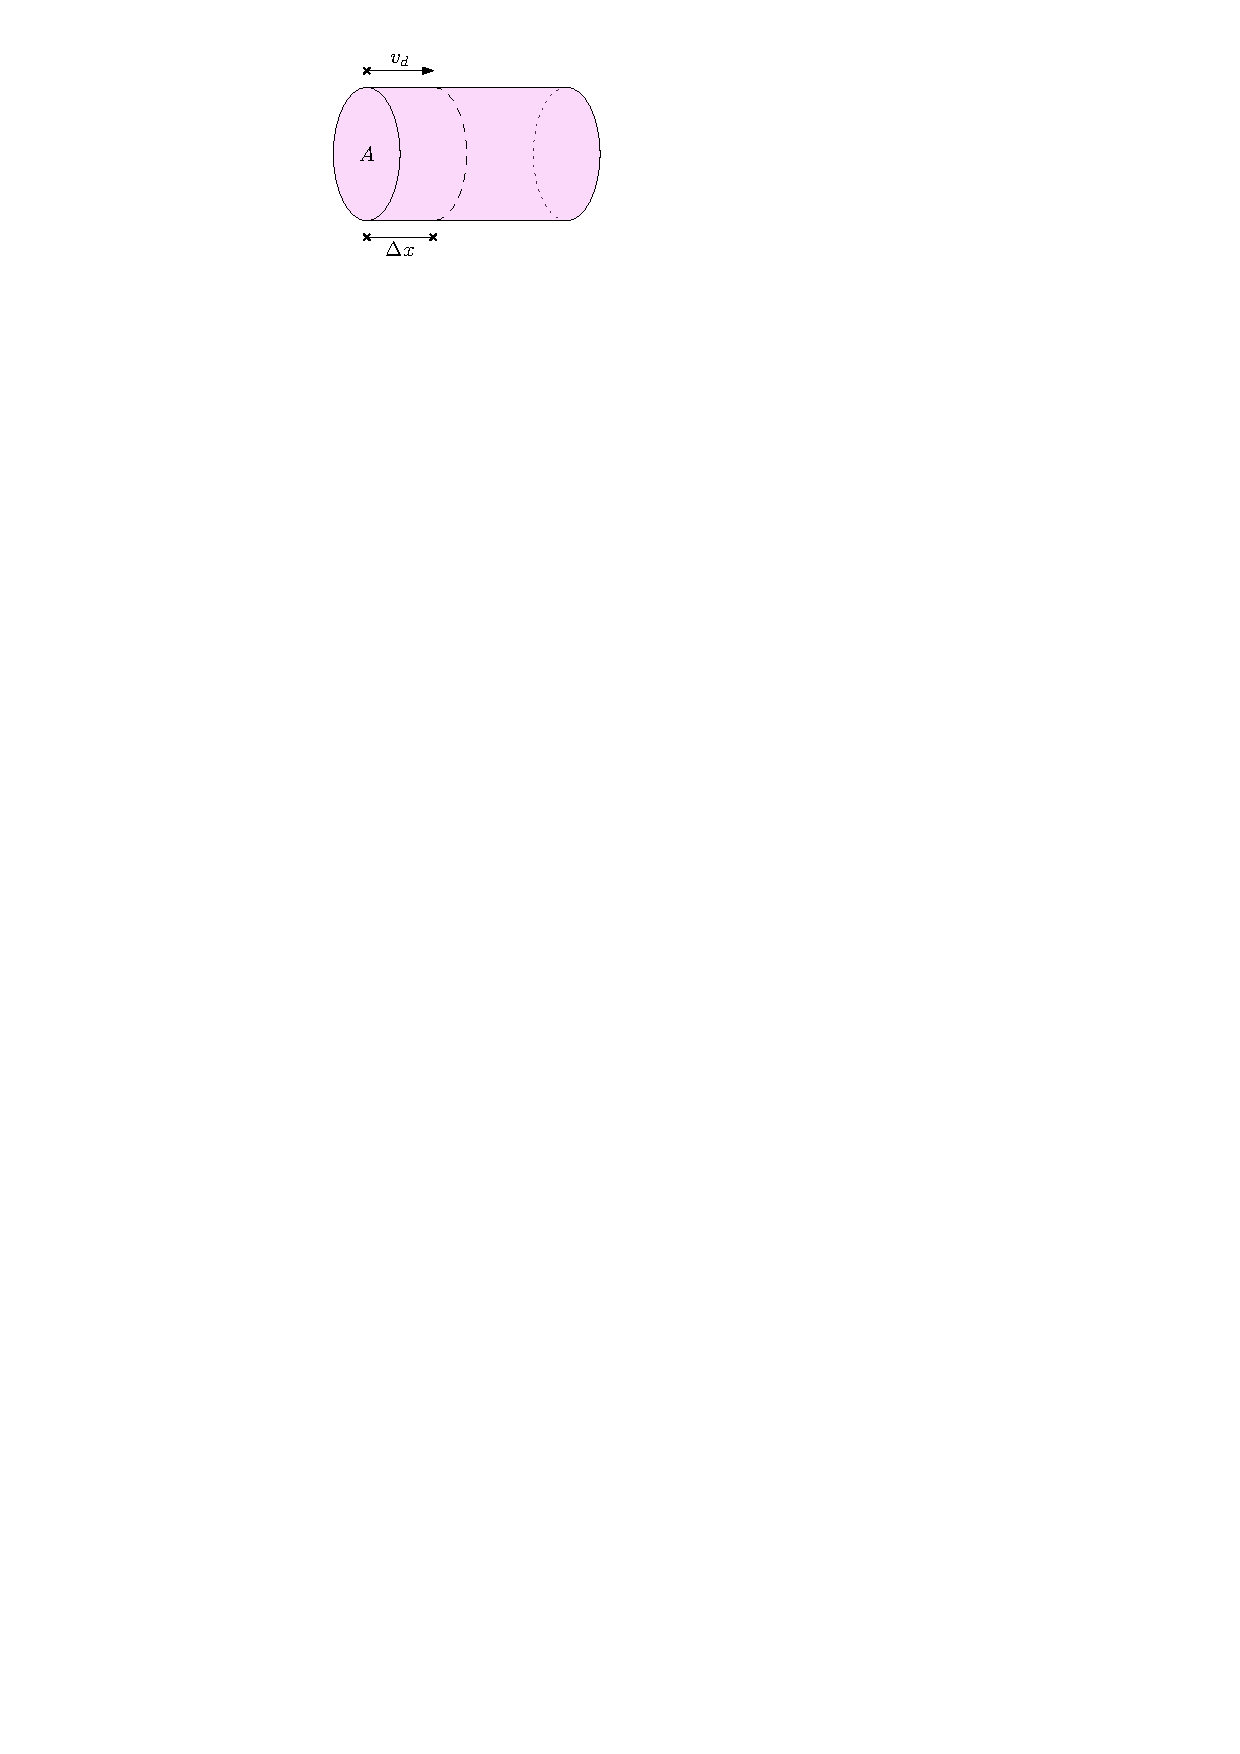
\includegraphics{figures/charge-carrier.pdf}
              \caption{A labeled diagram of a charge capacitor}
            \end{figure}
        \end{itemize}
      \item \textbf{capacitive discharging}
        \begin{figure}[H]
          \centering
          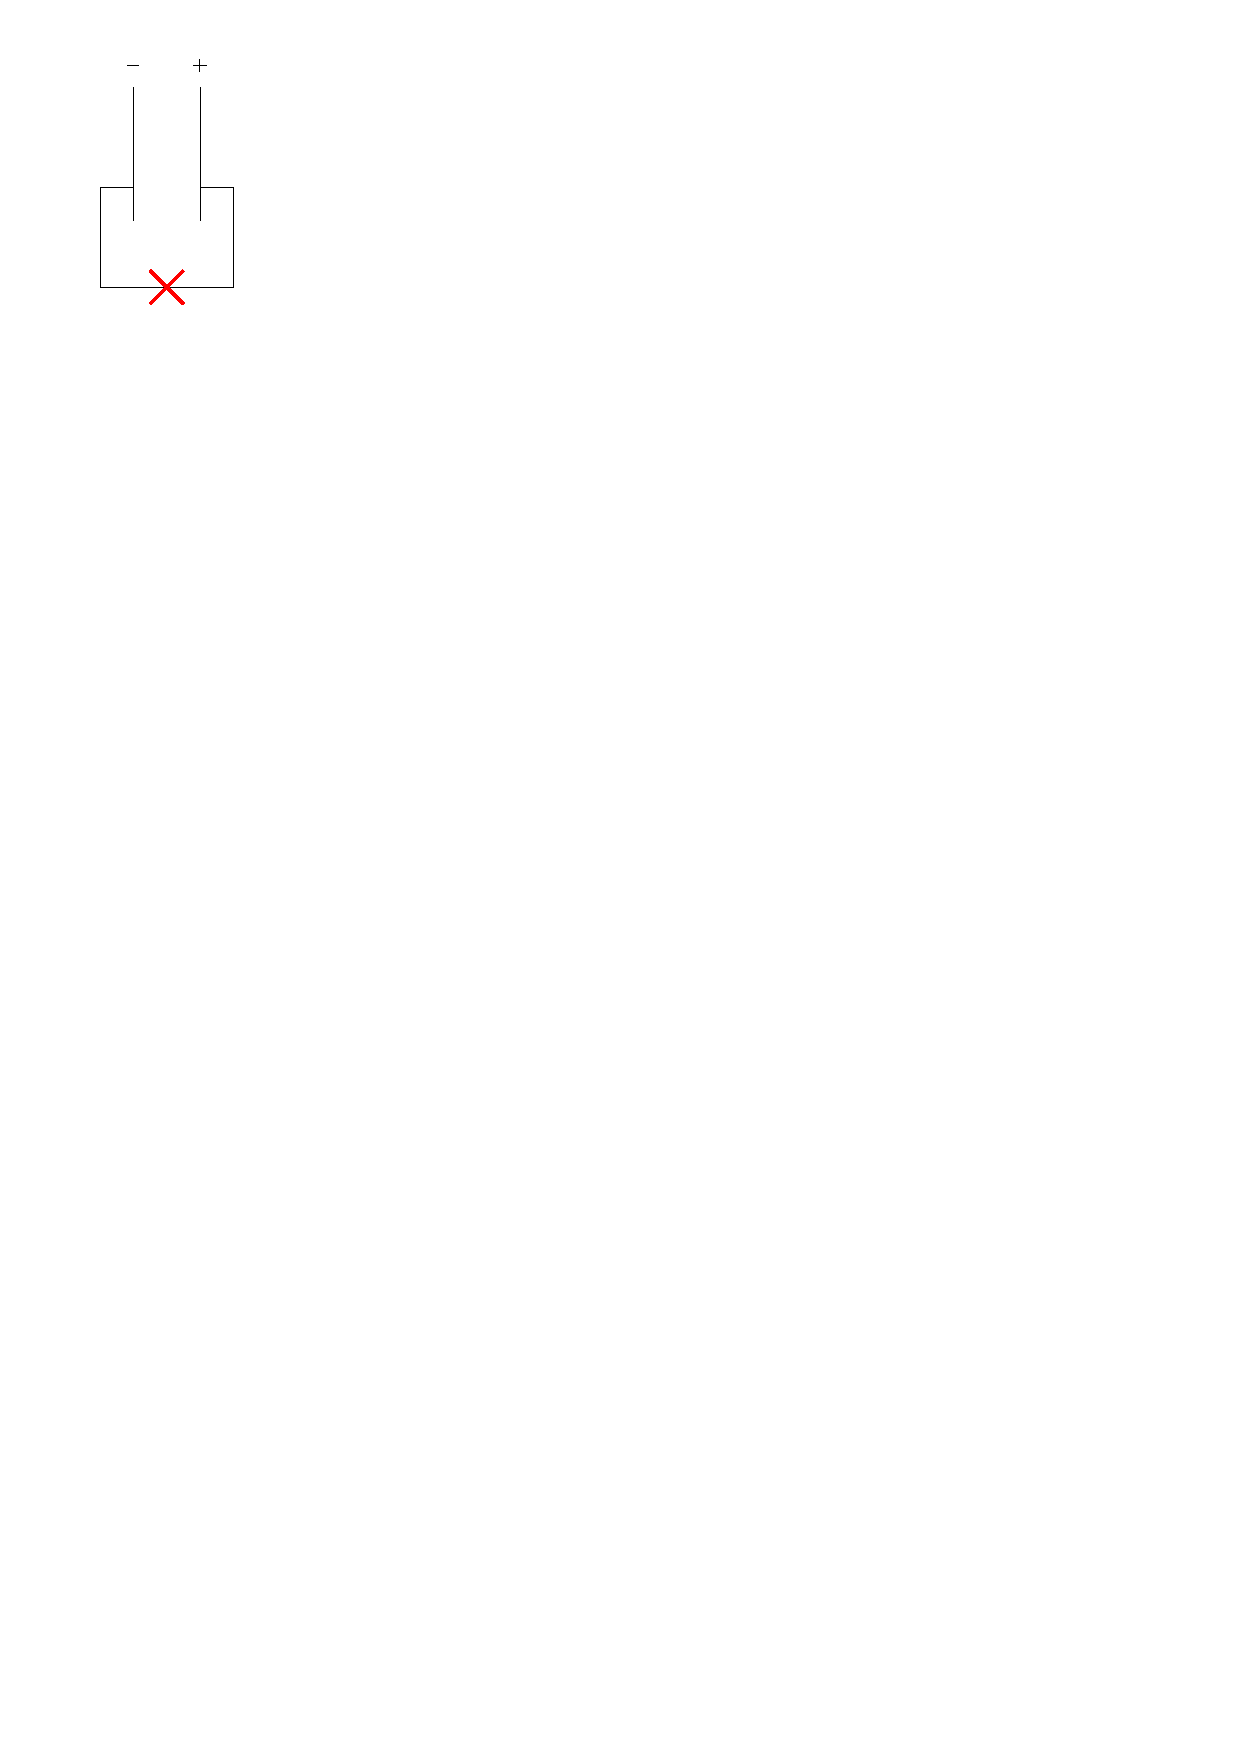
\includegraphics{figures/discharged-capacitor.pdf}
          \caption{A diagram of a discharged capacitor}
        \end{figure}
        \begin{itemize}
          \item discharge occurs immediately
          \item wire heats up
        \end{itemize} 
        \begin{figure}[H]
          \centering
          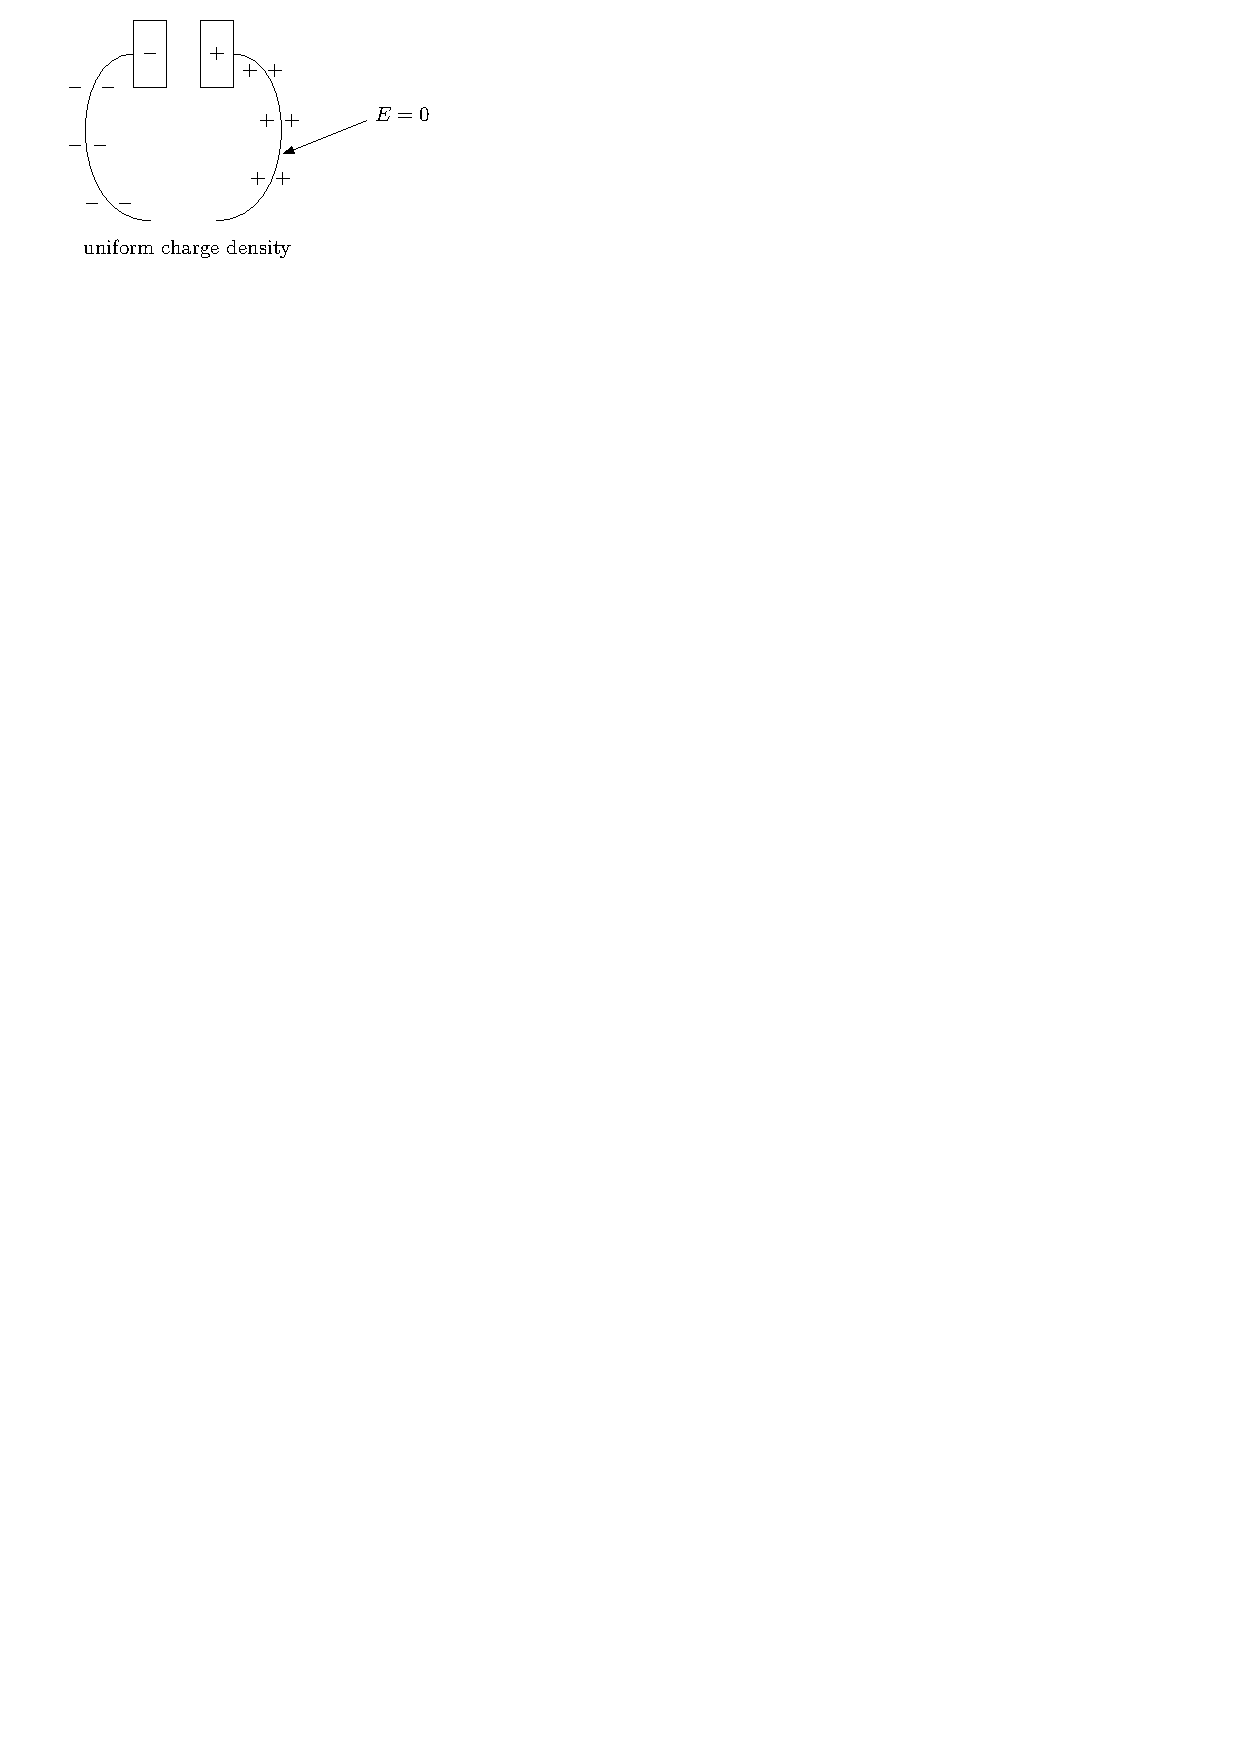
\includegraphics{figures/discharged-capacitor-2.pdf}
          \caption{A discharged capacitor with uniform charge density}
        \end{figure}
      \item \textbf{batteries}
        \begin{figure}[H]
          \centering
          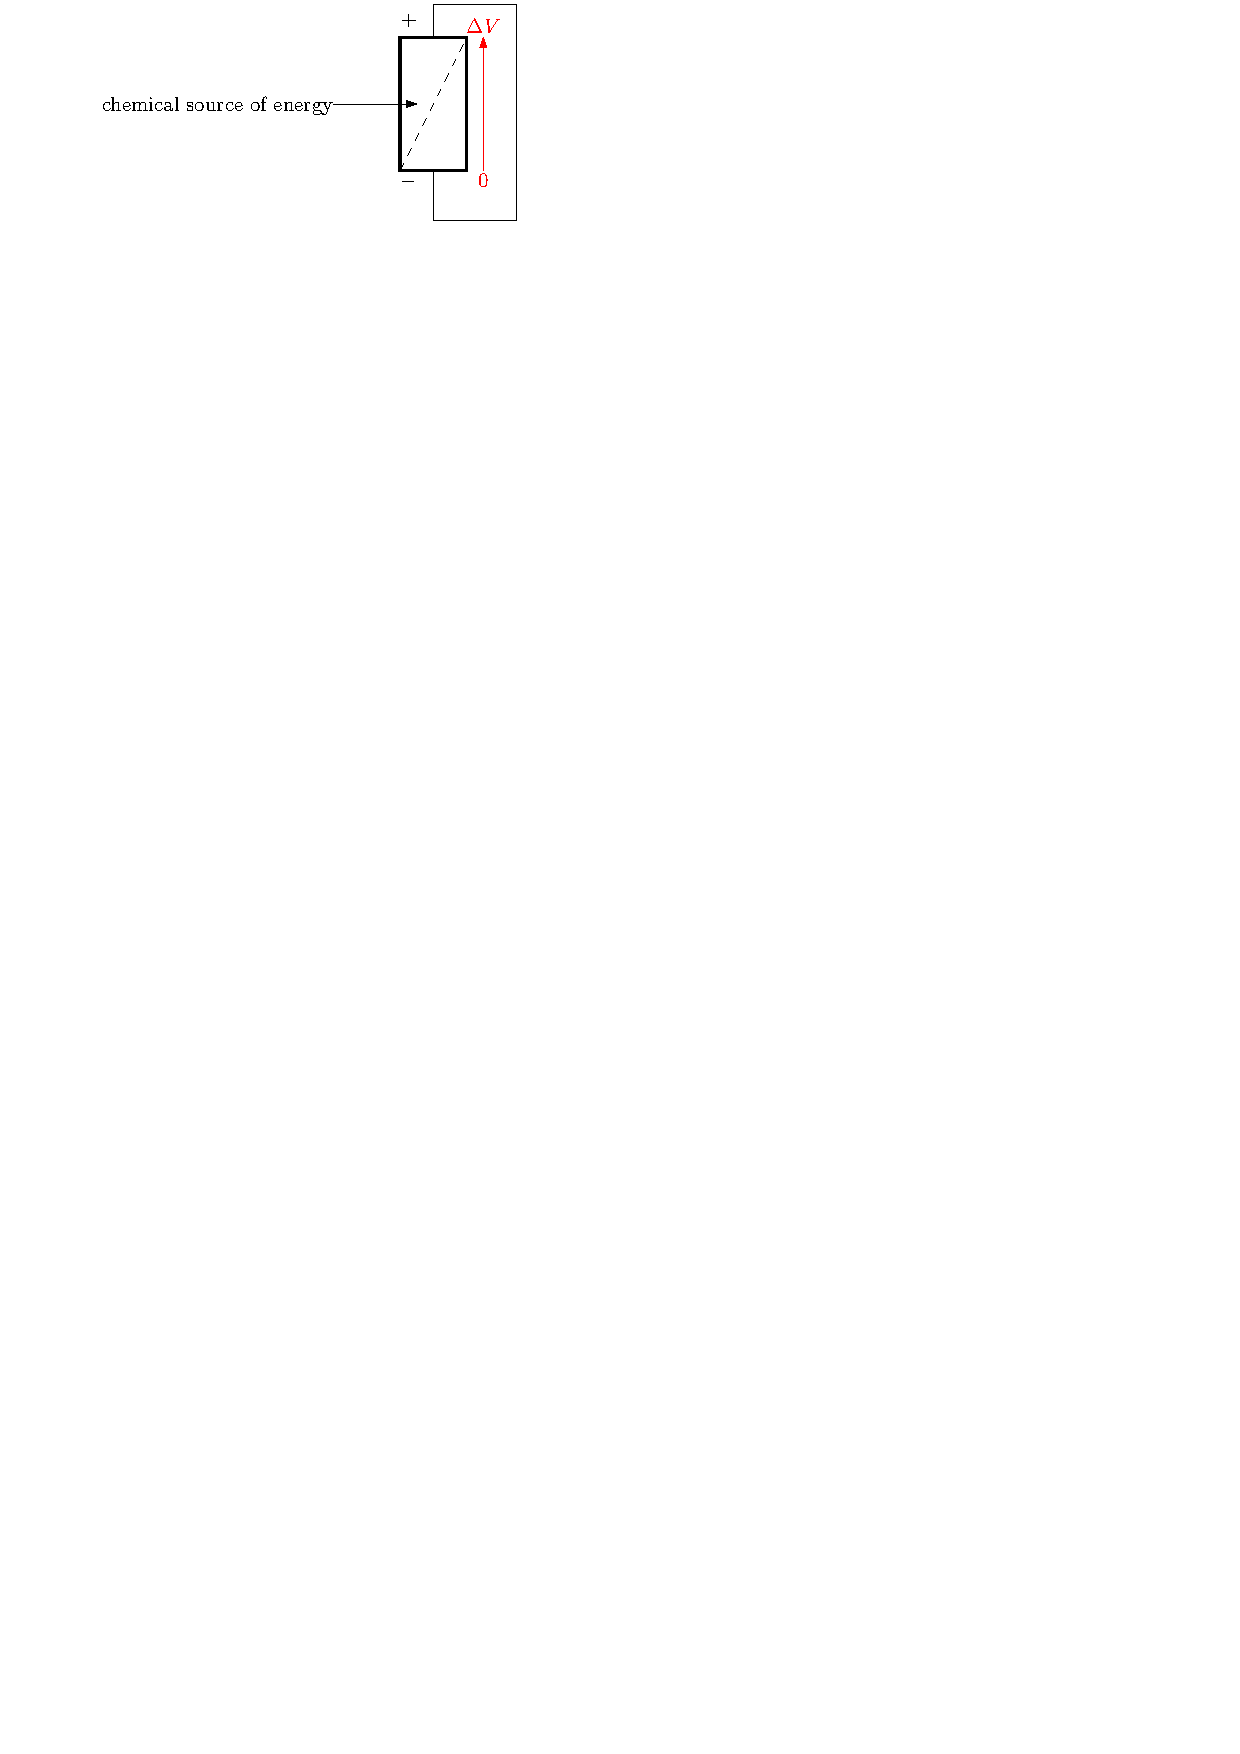
\includegraphics{figures/battery.pdf}
          \caption{A diagram of how a battery changes voltage}
        \end{figure}
        \begin{figure}[H]
          \centering
          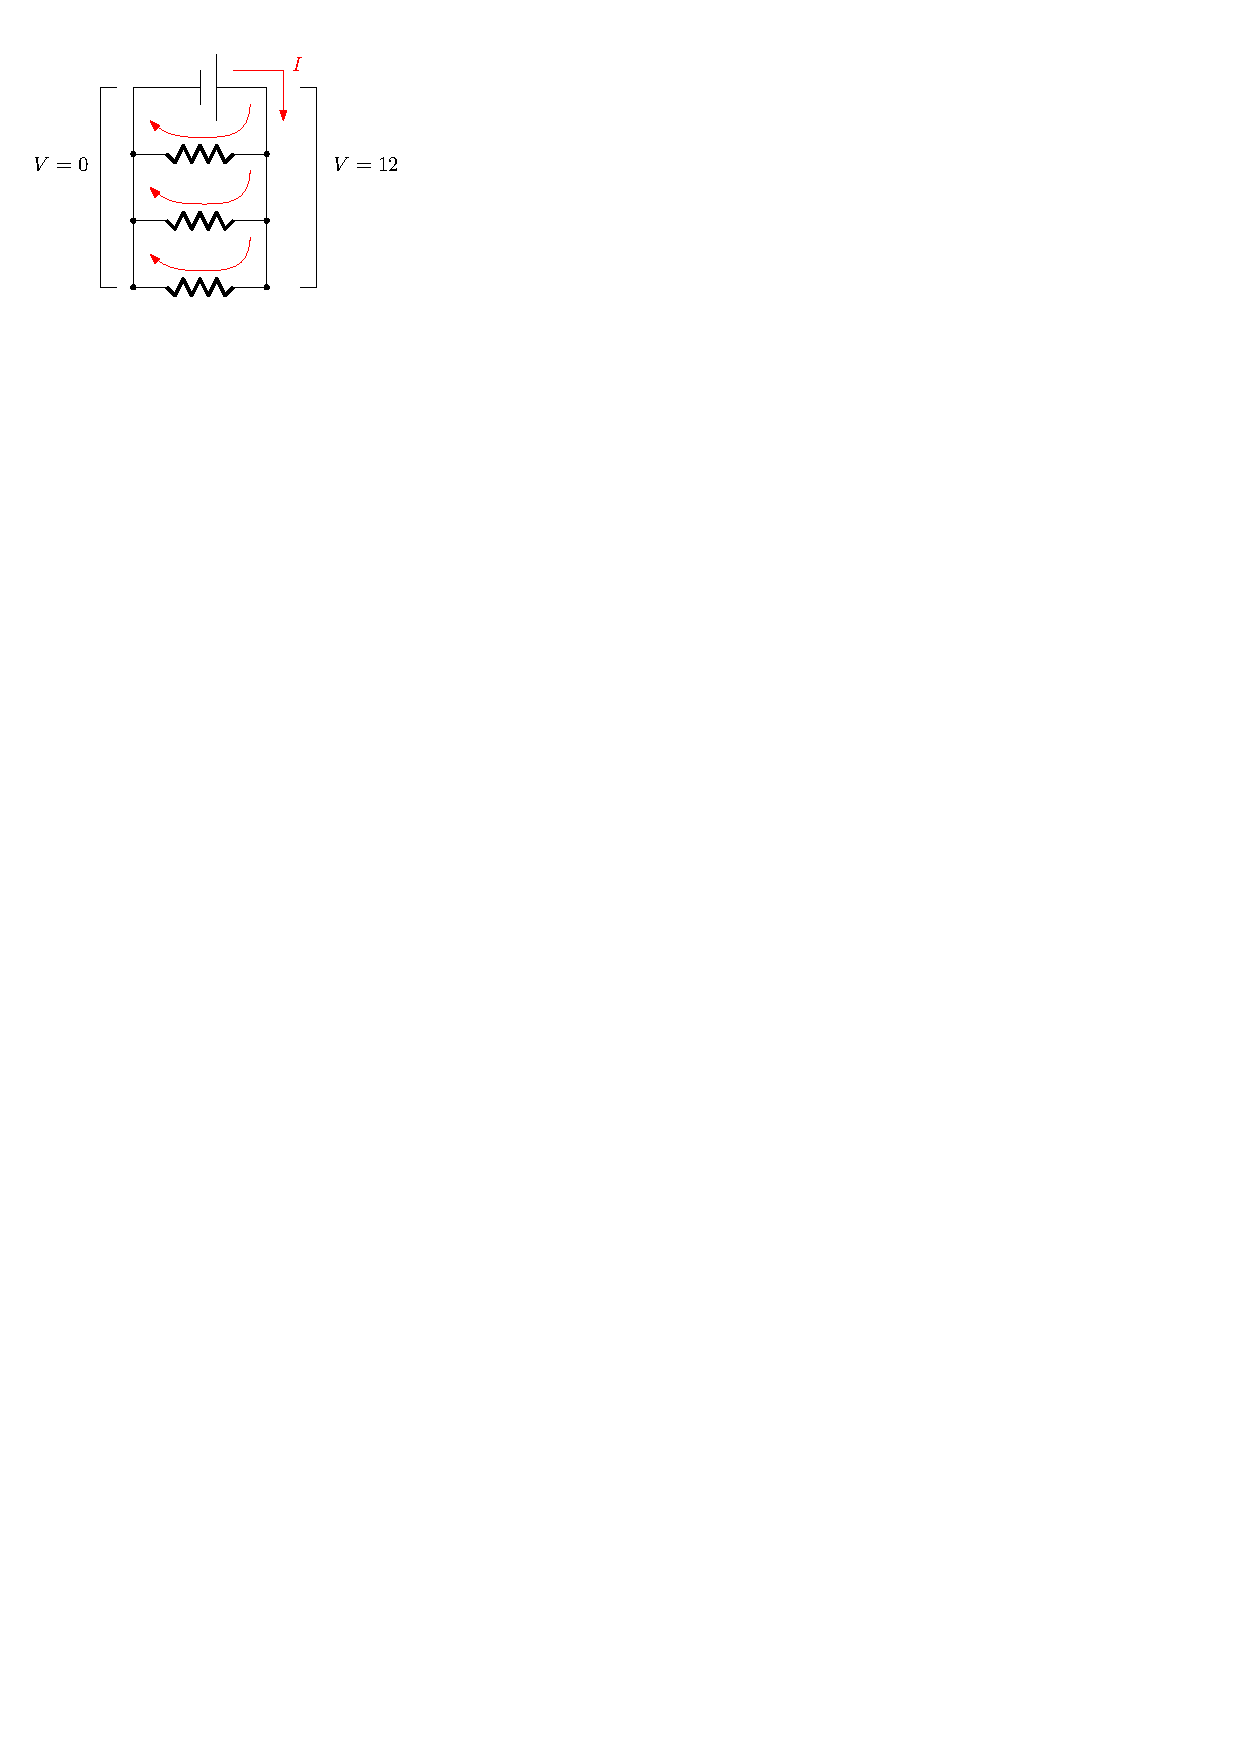
\includegraphics{figures/bat-change-v.pdf}
          \caption{A circuit with a battery and resistors, demonstrating the change in $V$}
        \end{figure}
        \begin{itemize}
          \item batteries work the same as capacitors
            \begin{itemize}
              \item provide a ``pathway back'' to $0$
            \end{itemize}
          \item \textbf{ideal batteries} have no internal resistance
          \item \textbf{non-ideal batteries} have internal resistance 
            \begin{figure}[H]
              \centering
              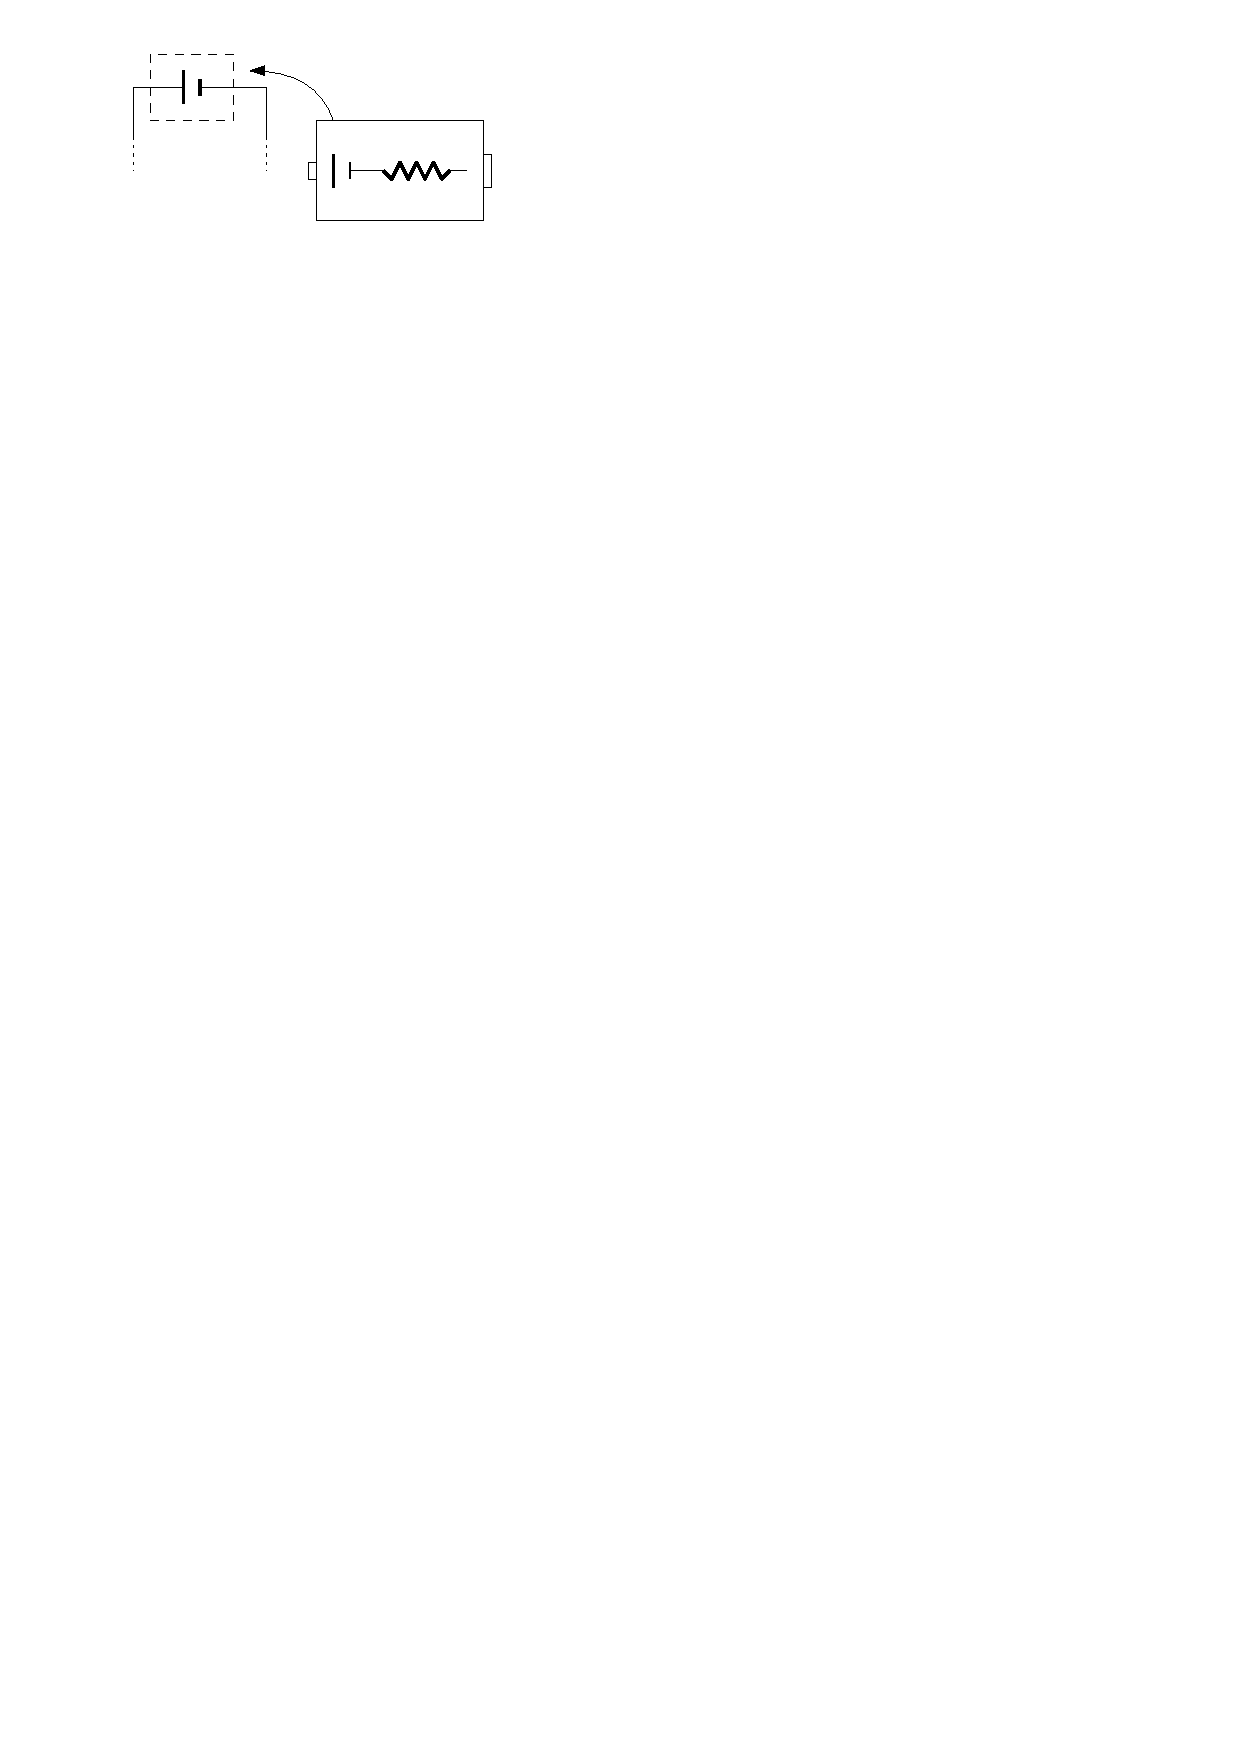
\includegraphics{figures/ir-battery.pdf}
              \caption{A battery with internal resistance (non-ideal)}
            \end{figure}
        \end{itemize}
    \end{itemize}
  \section{Capacitors, cont.}
    \begin{tabularx}{\textwidth}{X | X | X}
      \textbf{Parallel} & \textbf{Series} & \textbf{Mix}\\
      \hline
      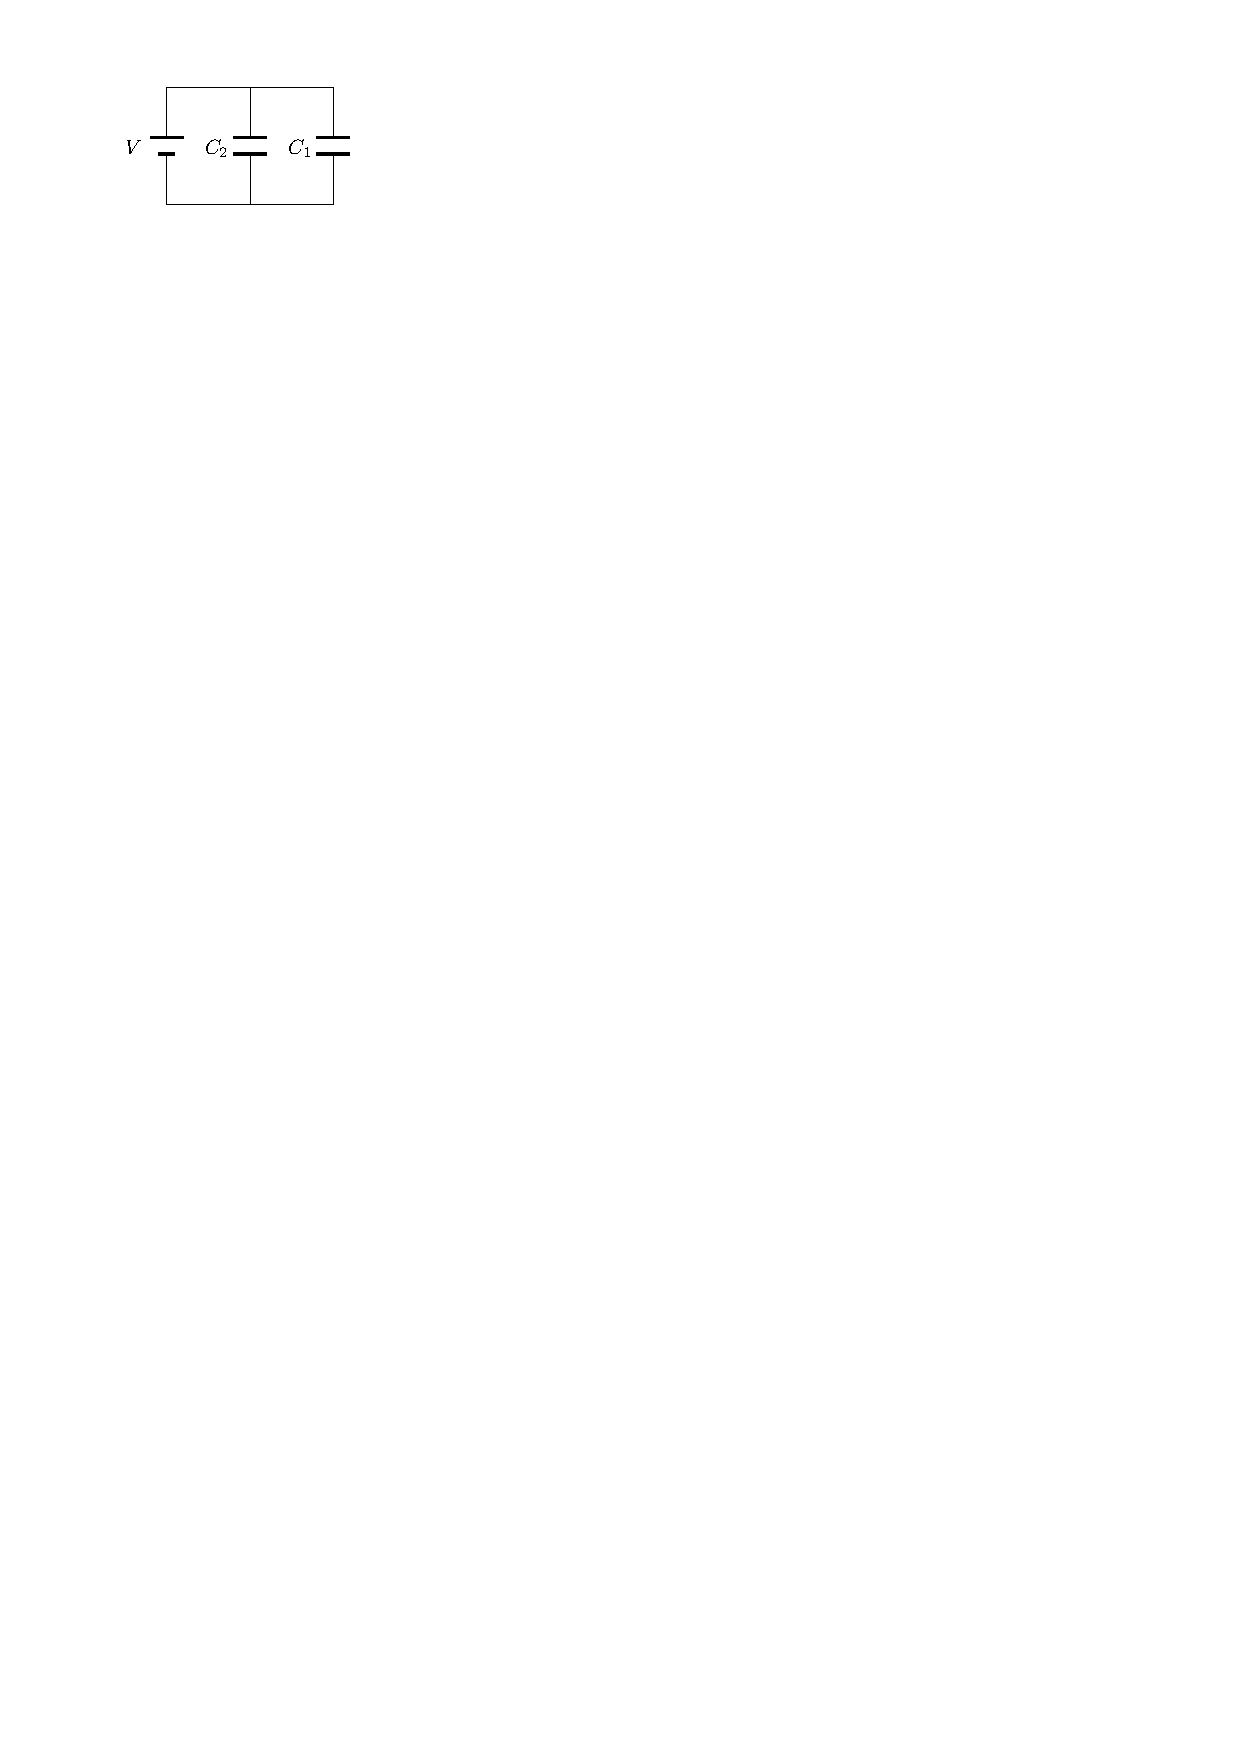
\includegraphics{figures/capacitors-in-parallel.pdf}\newline
      
      &
      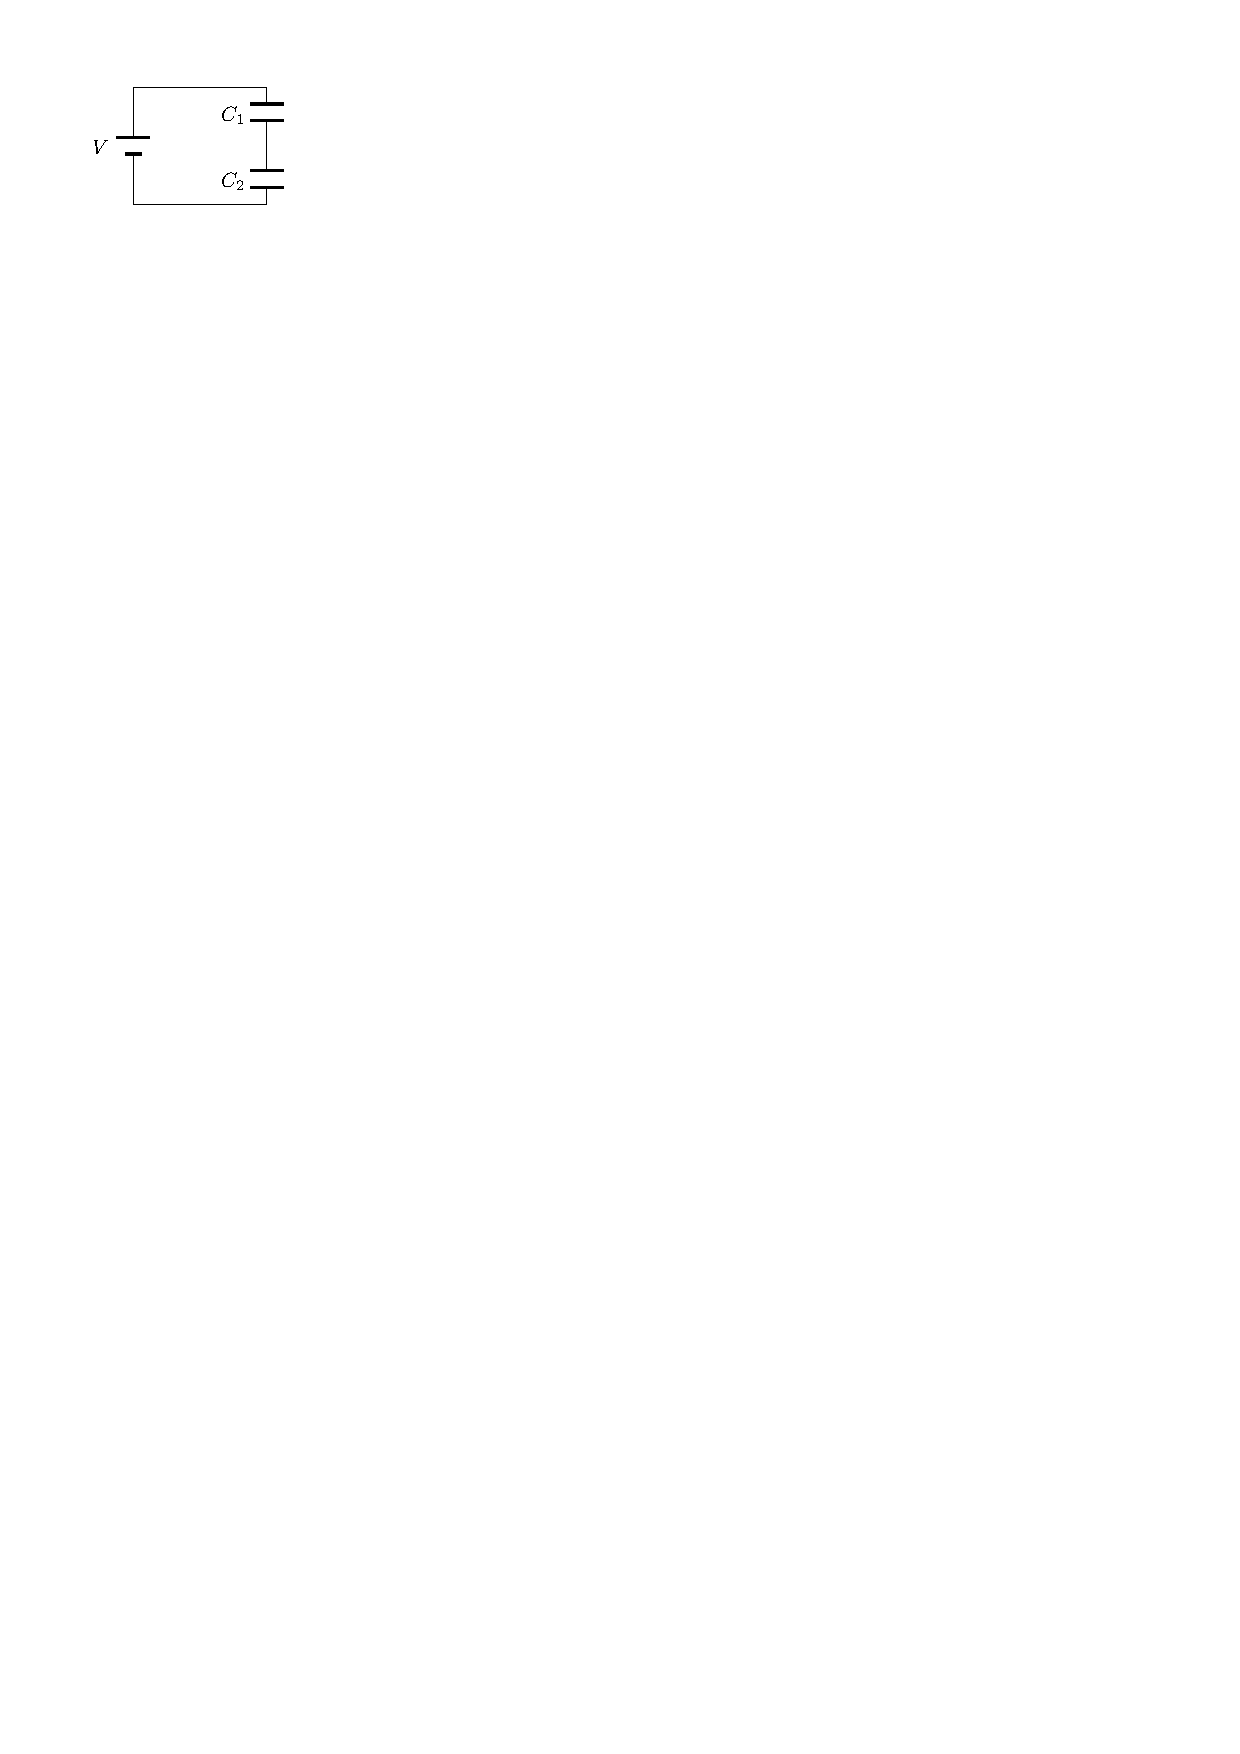
\includegraphics{figures/capacitors-in-series.pdf}
      &
      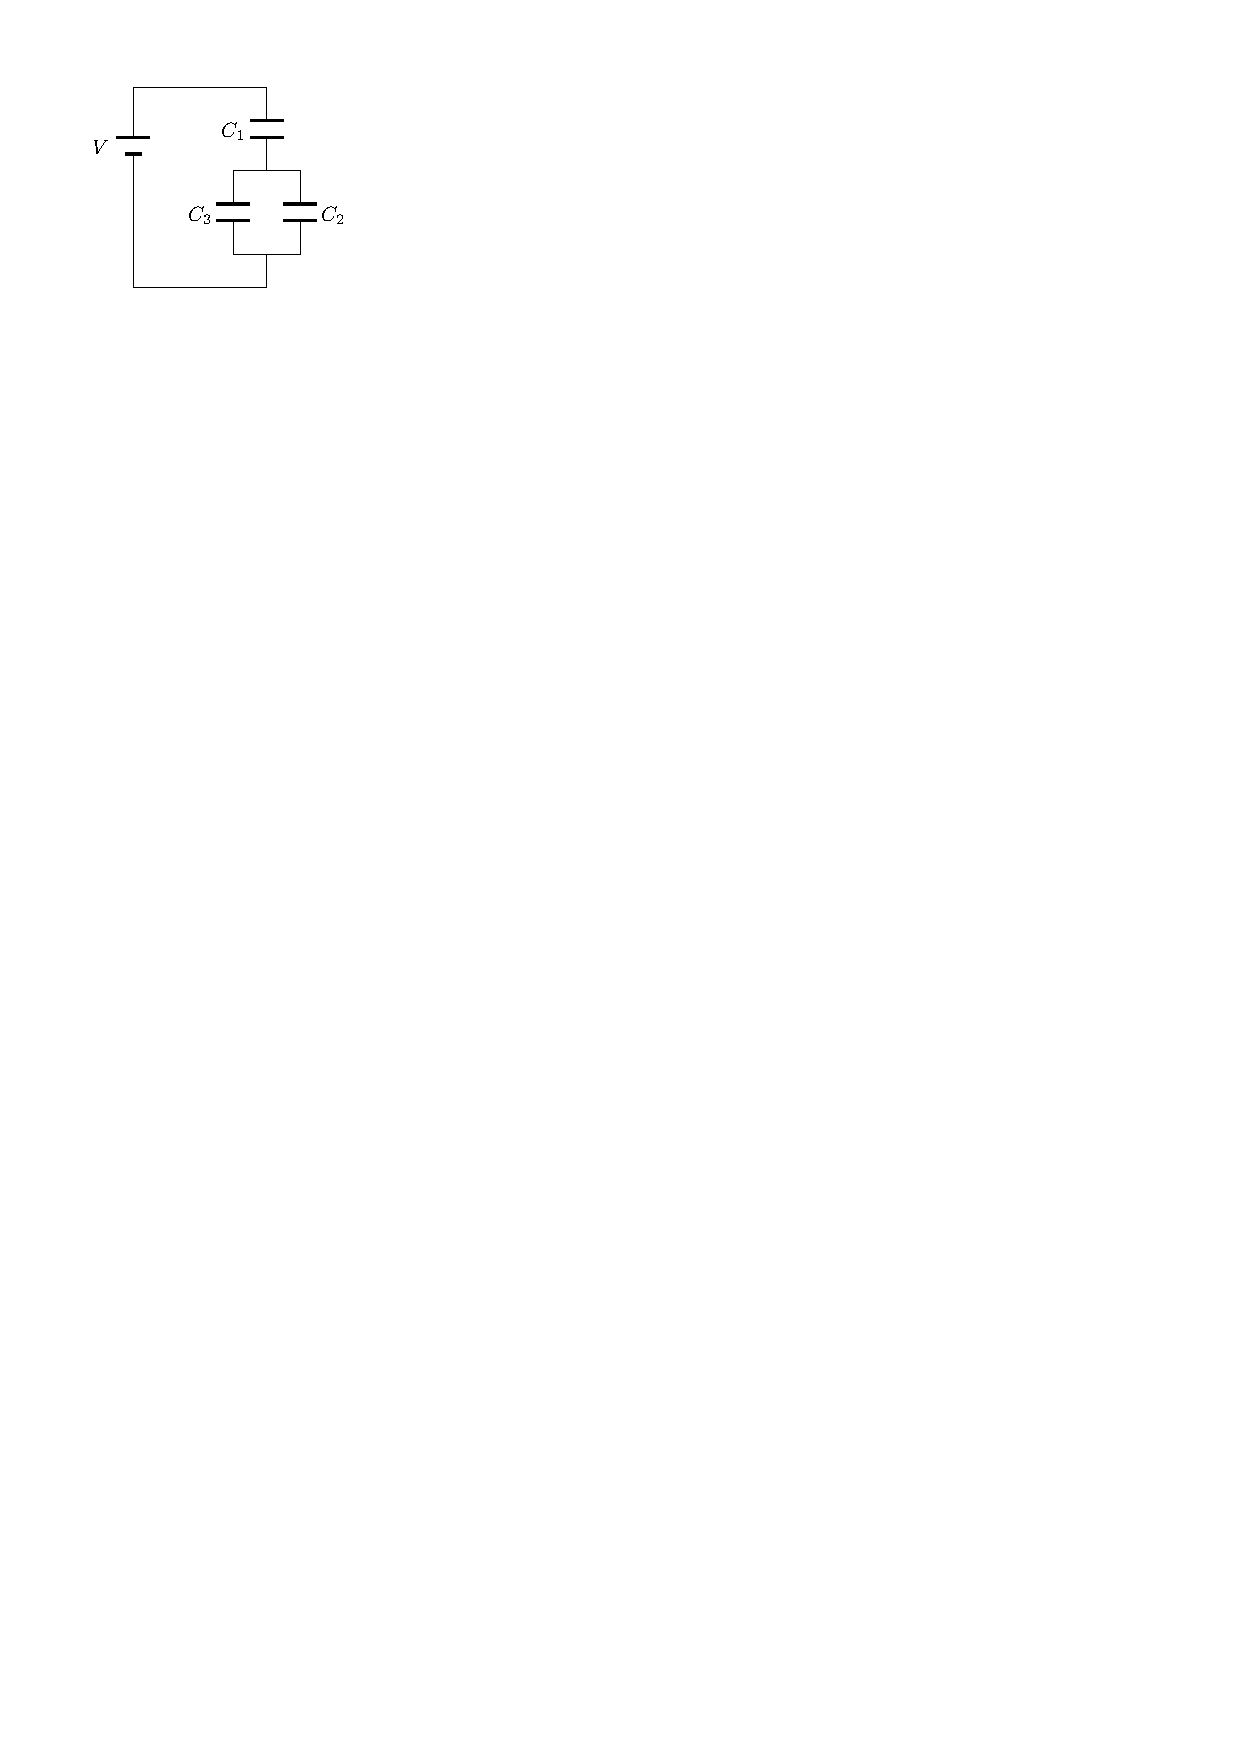
\includegraphics{figures/capacitors-in-mix.pdf}
    \end{tabularx}
    \subsection{Discharging a Capacitor}
    \begin{tabularx}{\textwidth}{ X | X }
      \textbf{Switch open} & \textbf{Right after switch is closed}\\ \hline
      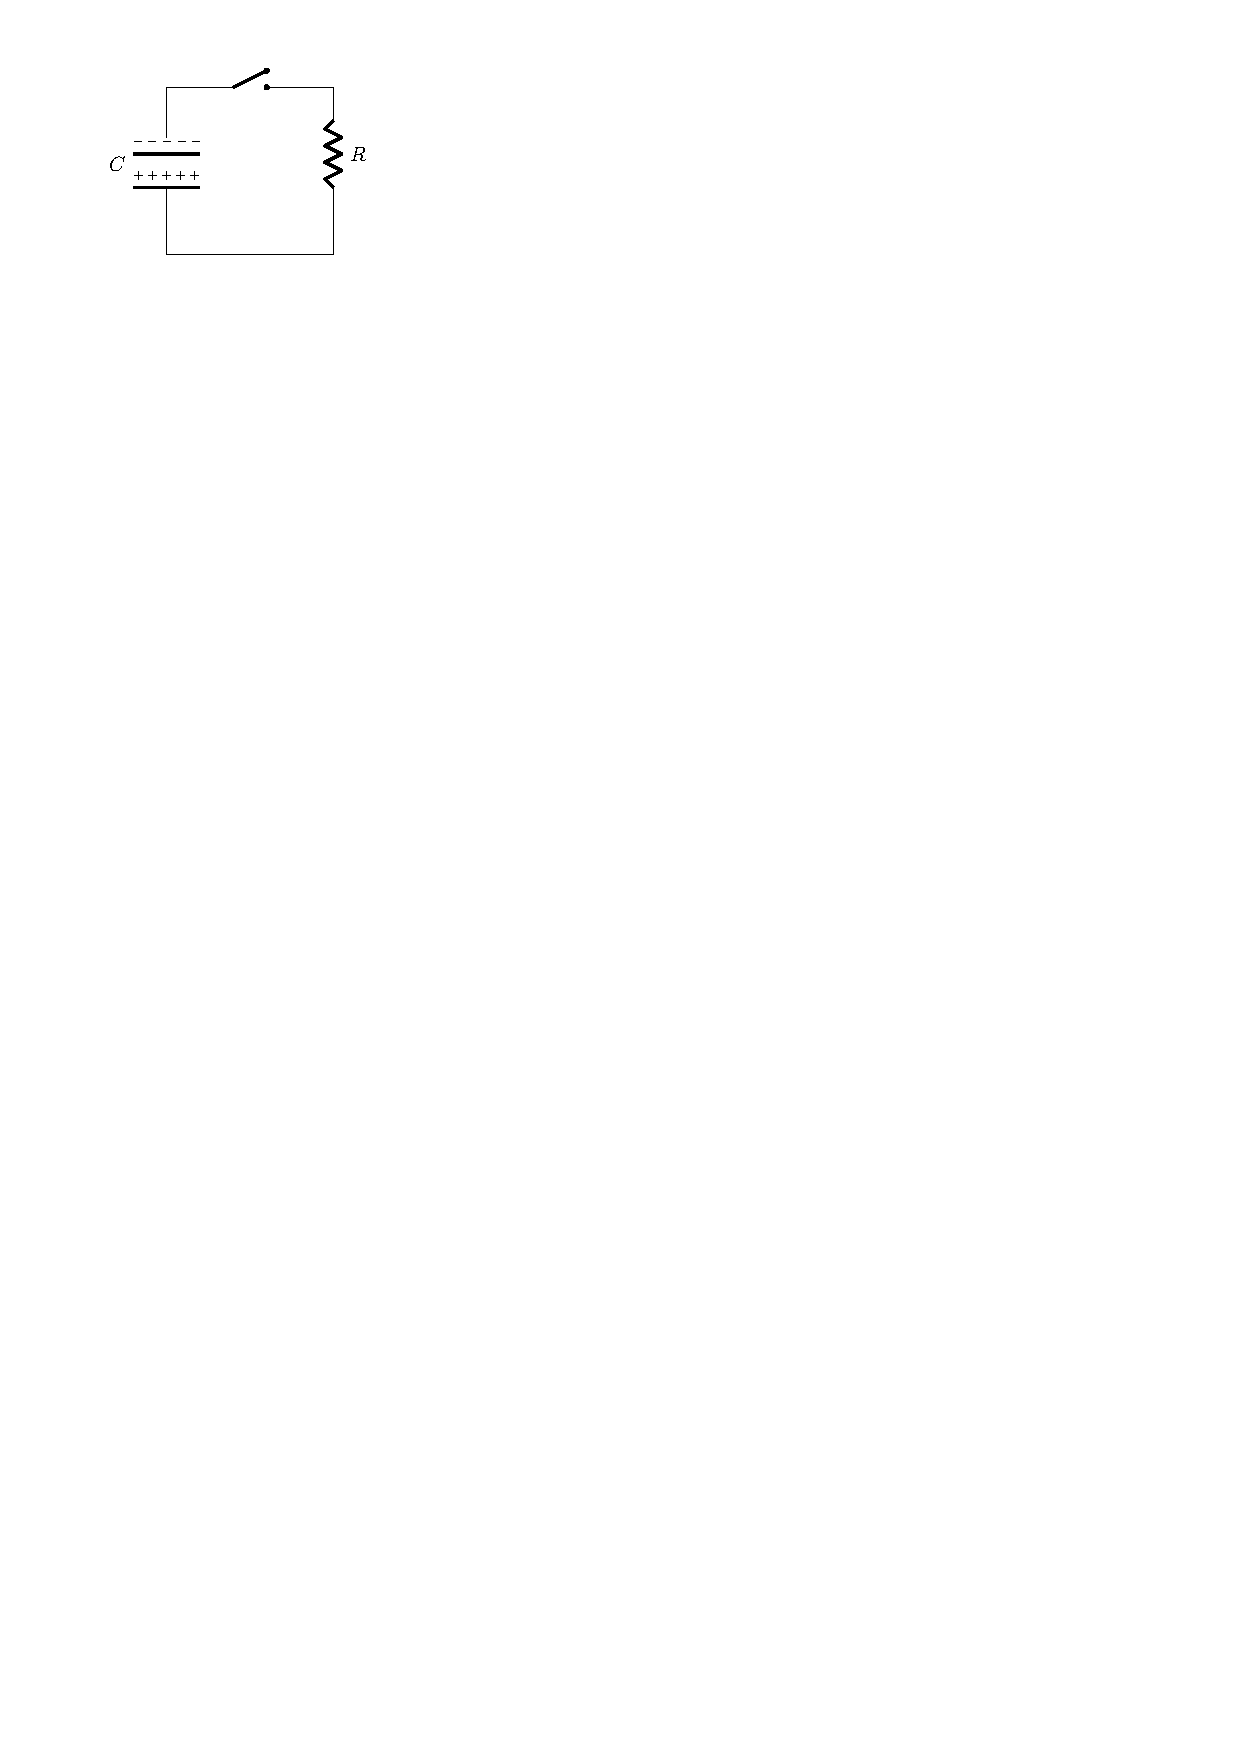
\includegraphics{figures/capacitor-discharge-open.pdf}
      {\begin{align*}
        Q_0 &=Q_{\mathrm{max}}\\
        I_0 &=0\\
        V_0 &=V_c=\text{max}=\dfrac{Q_0}{C}
      \end{align*}}
      &
      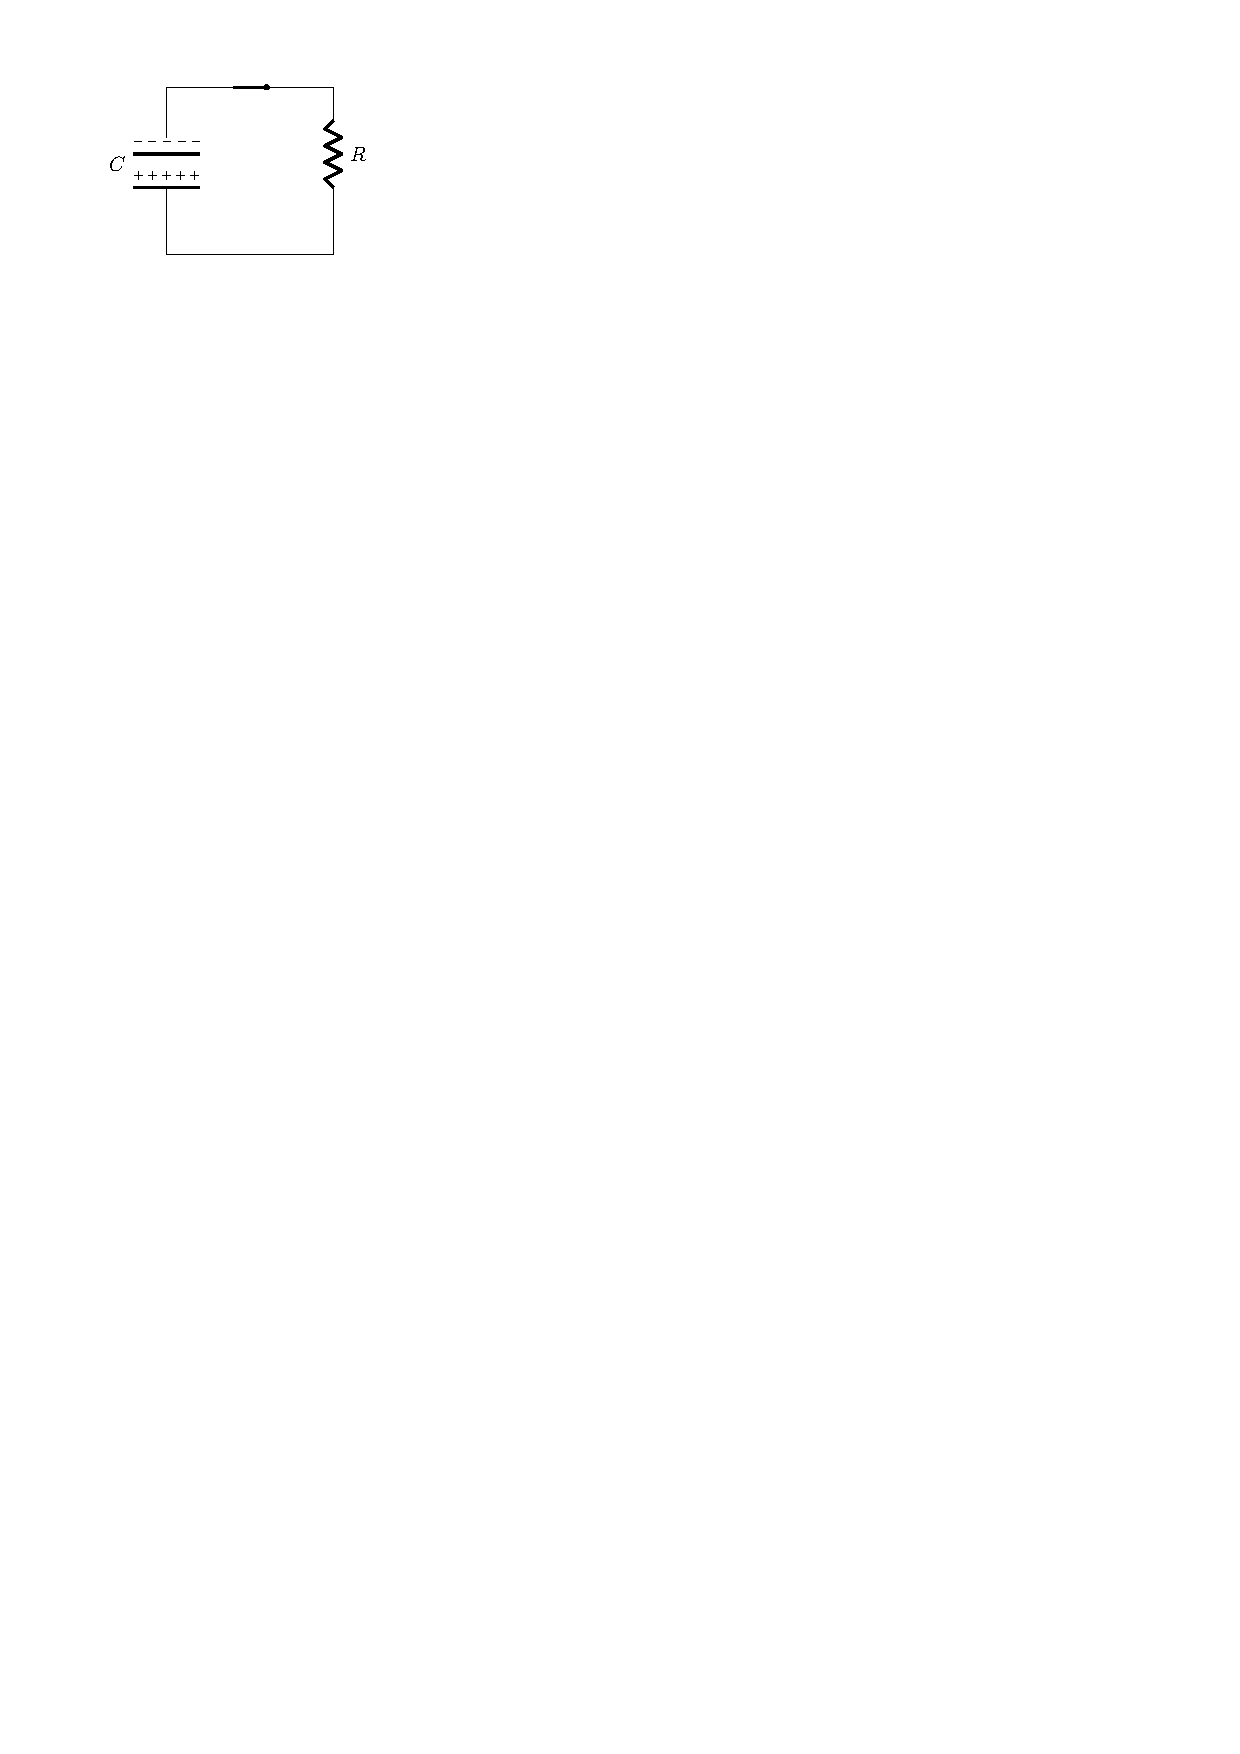
\includegraphics{figures/capacitor-discharge-closed.pdf}\newline
      $i$\newline
      $Q$ leaving $C$ get $i=-\dfrac{\dd{Q}}{\dd{t}}$\newline
      As $V_C\downarrow Q\downarrow I\downarrow$\newline
      $I_0=\mathrm{max}$\newline
      $V_C=\dfrac{Q}{C}$
    \end{tabularx}
    \begin{itemize}
      \item \textbf{loop rule}
        \begin{align*}
          V_c-IR&=0\\
          V_c-\left(-\dfrac{\dd{Q}}{\dd{t}}\right)R&=0\\
          \dfrac{1}{R}\left(\dfrac{Q}{C}+\dfrac{\dd{Q}}{\dd{t}}R\right)&=0\\
          \dfrac{Q}{RC}+\dfrac{\dd{Q}}{\dd{t}}&=0\\
          \dfrac{\dd{Q}}{Q}&=-\dfrac{1}{RC}\dd{t}
        \end{align*}
        then integrate...
        \begin{align*}
          \int_{Q_{\mathrm{max}}}^{Q} \dfrac{1}{Q} \dd{Q} &= -\dfrac{t}{RC}\\
          \ln(Q )\bigg|_{Q_{\mathrm{max}}}^Q&=-\dfrac{t}{RC}\\
          \ln(Q) -\ln(Q_{\mathrm{max}})&=\hskip 4mm {}^\wedge
        \end{align*}
        then simplify...
        \begin{align*}
          \ln\left(\dfrac{Q}{Q_{\mathrm{max}}}\right)&=-\dfrac{t}{RC}\\
          \cancel{\ln}\left(\dfrac{Q}{Q_{\mathrm{max}}}\right)&=e^{-{t}/{RC}}\\
          Q&=Q_{\mathrm{max}}\cdot e^{-{t}/{RC}}\\
          \Aboxed{RC&=\tau}
        \end{align*}
        \begin{figure}[H]
          \centering
          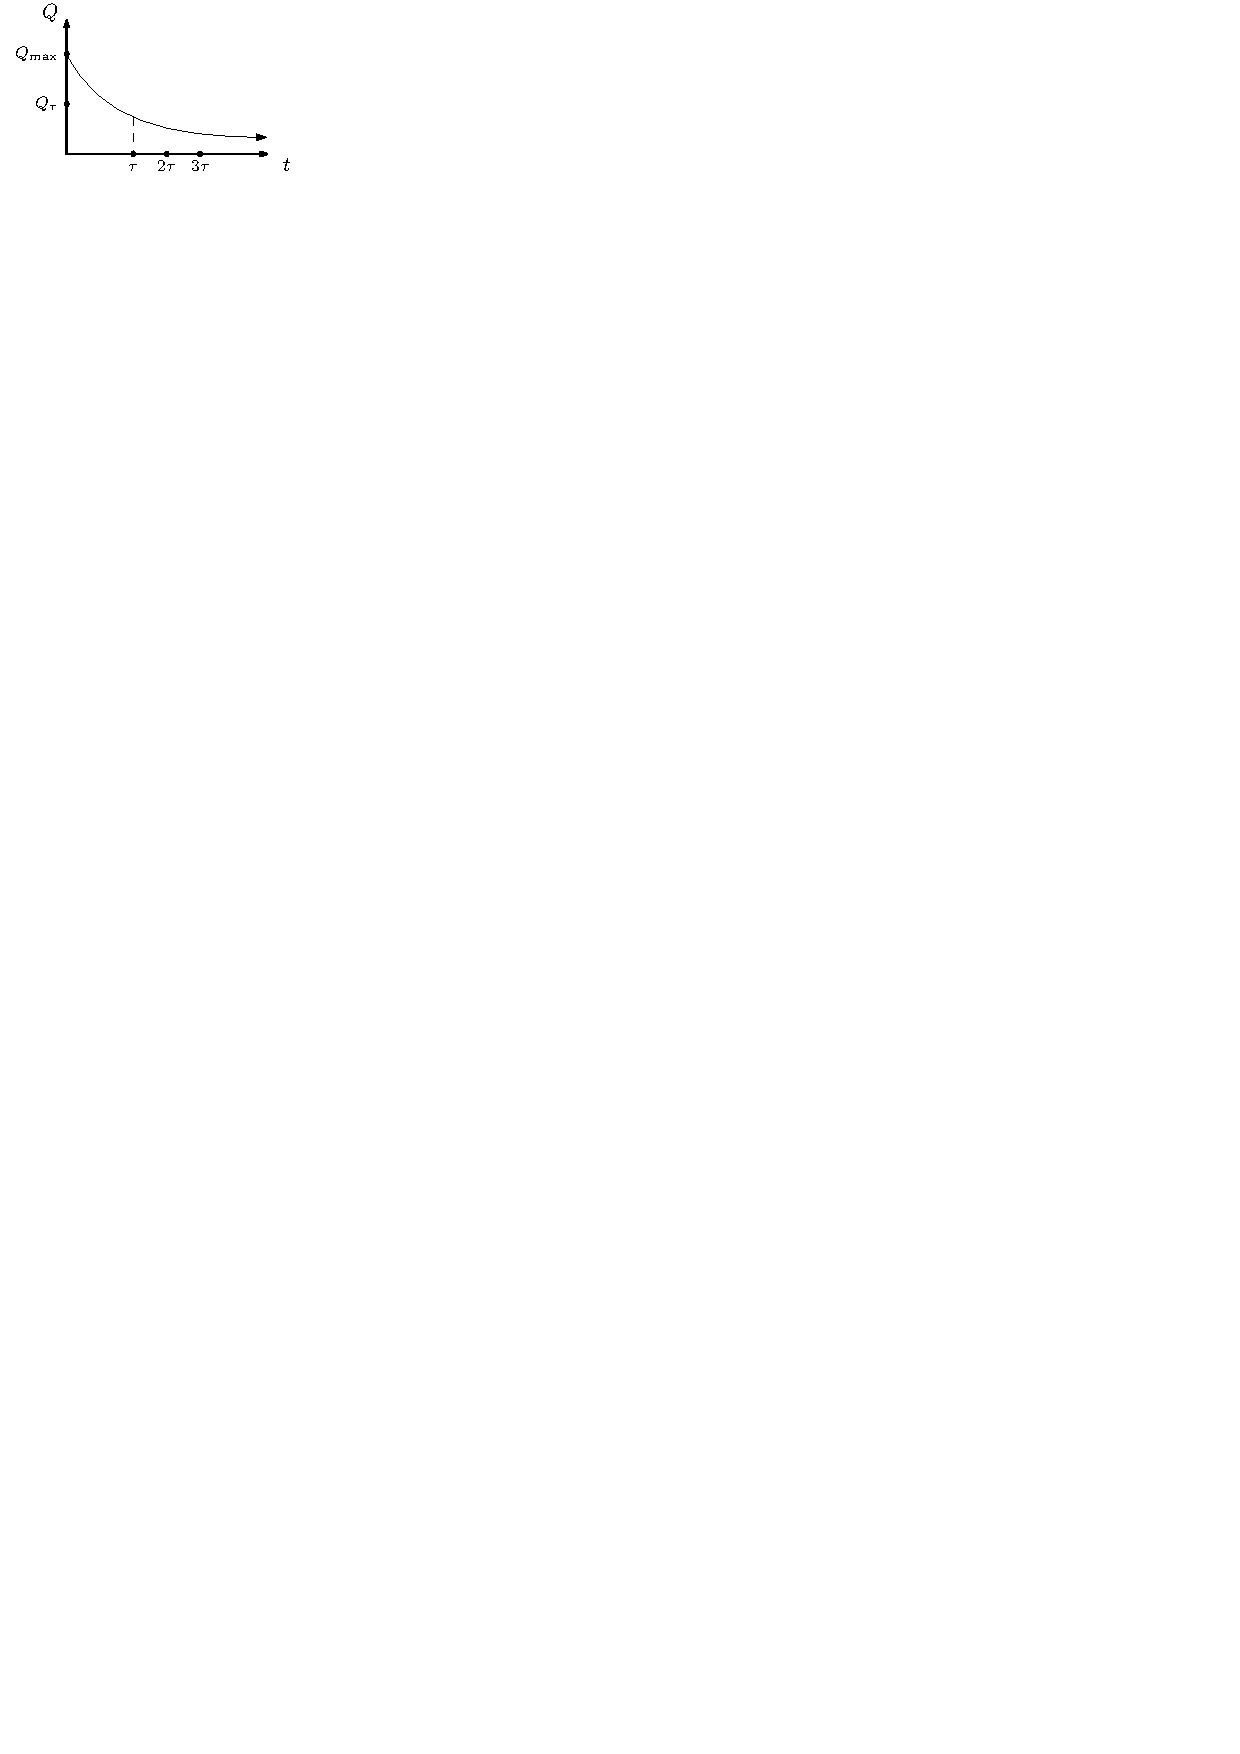
\includegraphics{figures/rc-charge-time.pdf}
          \caption{Charge over time in an RC circuit}
        \end{figure}
    \end{itemize}
\end{document}